\begin{frame}[t]{Traditional Numerical Methods in Geophysics}
\visible<1-3>{Main idea behind traditional inversion methods
\vspace{0.2cm} 
\begin{itemize}
\item $\rho$ are the resistivity values
\vspace{0.2cm} 
\item $H(\rho)$ is the set of simulated measurements
\vspace{0.2cm} 
\item $M$ is a set of measurements
\vspace{0.2cm} 
\end{itemize}}

\visible<2-3>{Find the resisitivity values $\rho$ whose simulated measurements $H(\rho)$ match the recorded set of measurements $M$}
\vspace{0.2cm} 

\visible<3>{
\textbf{Iterative scheme:}
\begin{equation}
\notag
\textup{Find $\rho^{(n)}$ that minimizes }C(\rho^{(n)}) :=|| H(\rho^{(n)}) - M ||,  \qquad \rho^{(n)} = \rho^{(n-1)} + \delta
\end{equation}
Simulated measurements $H(\rho)$ $\Longrightarrow$ Solve the forward problem!}
\end{frame}


\begin{frame}{Traditional Numerical Methods in Geophysics}
\begin{thebibliography}{1}
\bibitem{paper1} \small{S. Bakr, D. Pardo, C. Torres-Verdín. Fast inversion of logging-while-drilling resistivity measurements
acquired in multiple wells. GEOPHYSICS, 82(3): E111-E120, 2017.}
\vspace{0.3cm}
\bibitem{paper2} D. Pardo and C. Torres-Verdín. Fast 1D inversion of logging-while-drilling resistivity
measurements for improved estimation of formation
resistivity in high-angle and horizontal wells. GEOPHYSICS, 80(2):E111-E124, 2015.
\vspace{0.3cm}
\bibitem{paper3} T. Günther,  C. Rücker and  K. Spitzer. Three-dimensional modelling and inversion of dc resistivity data incorporating topography — II. Inversion. Geophysical Journal International, 166(2): 506–517, 2006.
\vspace{0.3cm}
\bibitem{paper4} O. Ijasan, C. Torres-Verdín, and W. Preeg. Inversion-based petrophysical interpretation of logging-while-drilling nuclear and resistivity measurements. GEOPHYSICS, 78(6):D473-D489, 2013.
\end{thebibliography}
\end{frame}



\begin{frame}{Traditional Numerical Methods in Geophysics}
\begin{columns}
\begin{column}{0.5\textwidth}
	\begin{figure}
	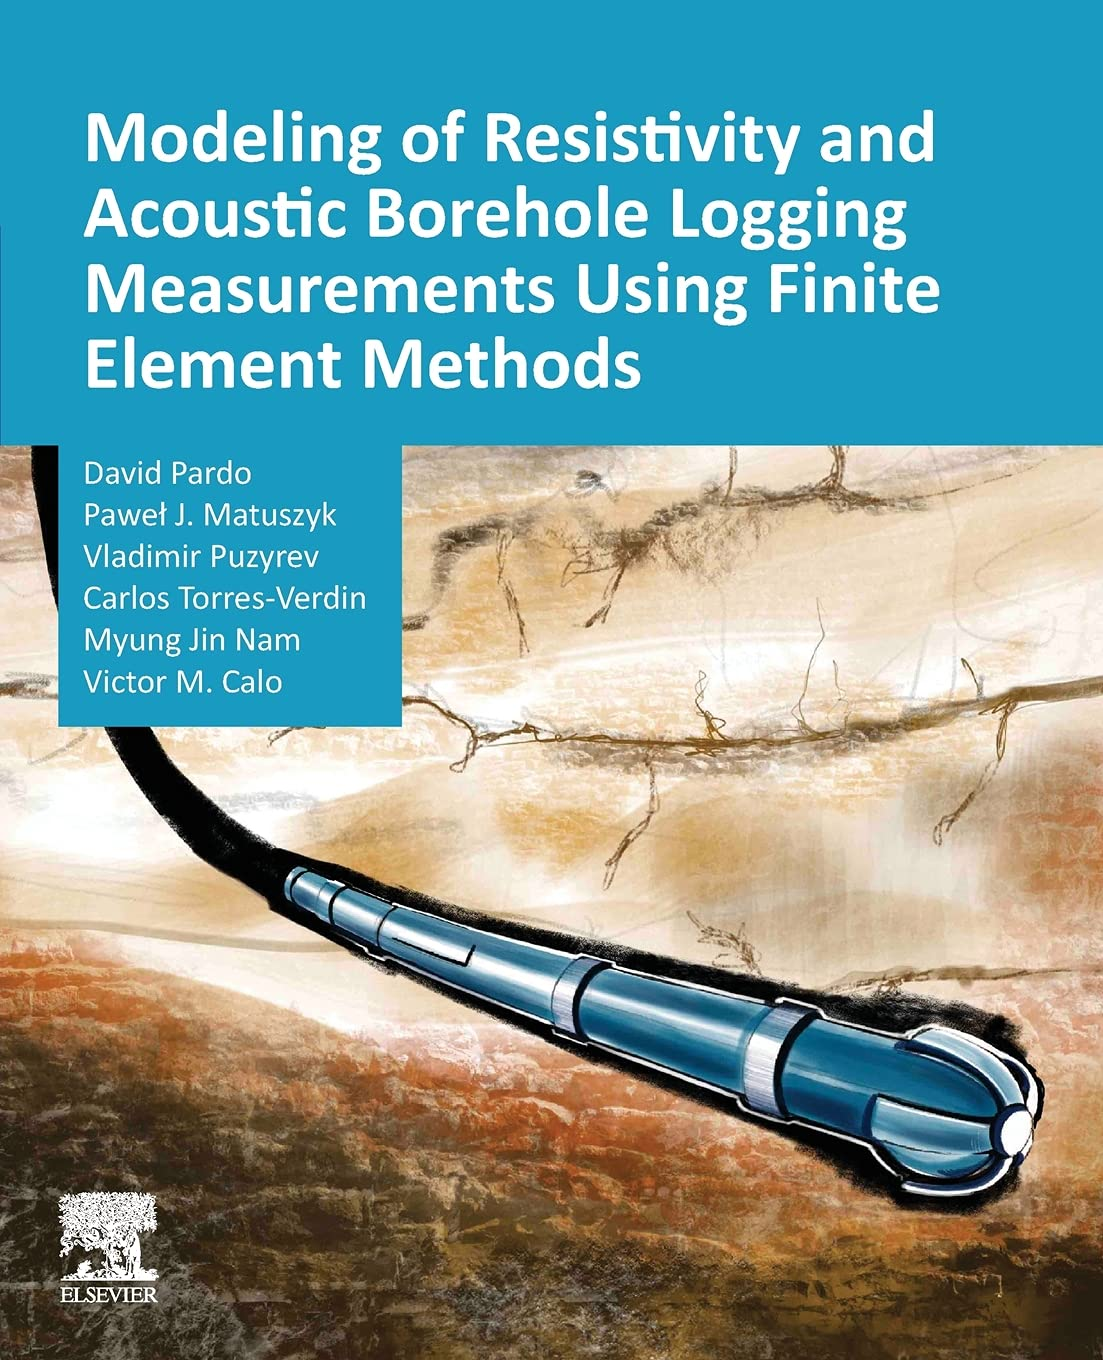
\includegraphics[scale=0.13]{Diapos/Intro/Figures/PardoBook.jpg}
	\end{figure}
	\hspace{0.9cm} {\small Published in 2021}
\end{column}
%
\begin{column}{0.5\textwidth}
\begin{itemize}
\item Finite Element method
\vspace{0.5cm}
\item Finite Difference method
\vspace{0.5cm}
\item Finite Volumes method
\vspace{0.5cm}
\item Integral methods
\vspace{0.5cm}
\item Semi-analytical methods
\end{itemize}
\end{column}
\end{columns}
\end{frame}

\begin{frame}{Traditional Numerical Methods}
\visible<1-2>{
\textbf{Limitations:}
\vspace{0.3cm}

Finite Element/Difference methods:
\vspace{0.3cm}
\begin{itemize}
\item Mesh dependent
\vspace{0.3cm}
\item Fine grids for better accuracy $\Rightarrow$ High computational cost
\vspace{0.3cm}
\end{itemize}
\vspace{0.3cm}
Integral methods:
\vspace{0.3cm}
\begin{itemize}
\item Design of fast and robust integration techniques
\vspace{0.3cm}
\item Dense matrices $\Rightarrow$ High computational cost
\end{itemize}
}
\vspace{0.3cm}
\visible<2>{\begin{center}
\textcolor{red}{Need for real-time borehole inversion}
\end{center}
}
\end{frame}



